\chapter{Introduction}


\section{Strongly Correlated material}

Modern solid-state physics tries to explain the physical properties of different materials such as simple metals, semiconductors and insulators. But some materials in which their $d$ and $f$ electron shells are not fully occupied and electrons occupy narrow orbitals show complicated properties \cite{Gabriel}. For example, transition metals V, Fe, Ni, and their oxides, or rare- earth metals such as Ce belong to this group. This situation, where there is an open $d$ or $f$ electron shell, increases the effect of the Coulomb interaction between the electrons. These materials with strong electron-electron interaction are strongly correlated systems \cite{Piers}. As mentioned before these materials show complicated and interesting features: phase transitions between magnetic order and superconductivity, appearance and disappearance of local magnetic moments, transport property anomalies \cite{Vladimir}. As example, some strongly correlated systems can be listed as below \cite{Piers}:

\begin{itemize}
    \item Cuprate superconductors, 
    \item Heavy-electron compounds,
    \item Fractional quantum Hall systems,
    \item Quantum dots,
    \item Cold atomic gases,
\end{itemize}

A huge number of strongly correlated materials have atoms which are not fully occupied in $d$ or $f$ orbitals. Heavy-electron materials are an excellent example of this group, the component of the electron fluid, which is extremely localized in $f$ orbitals, create magnetic moments. The driving force for the strongly correlated electrons systems is provided by the interplay of the conduction electrons with localized magnetic moments \cite{Piers}.
\begin{figure}[ht]
\centering
    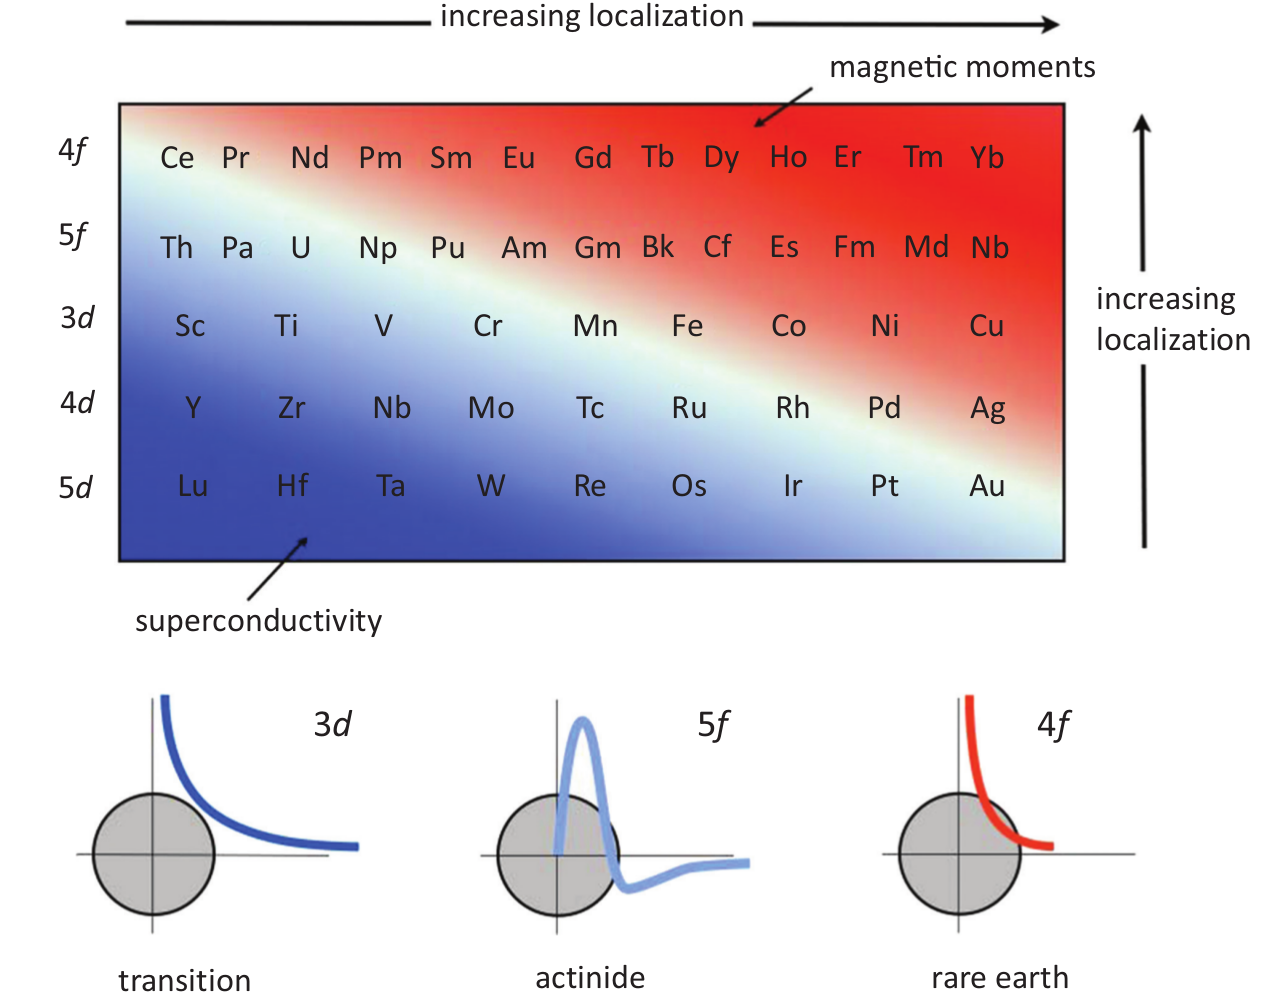
\includegraphics[width=1\linewidth]{fig1/1.png}
    
\caption{Kmetko-Smith diagram, displaying the behaviour of elements based on increasing electron localization in $d$ and $f$ electron orbitals \cite{Piers}. \label{fig:periodic table}}
\end{figure} 

The behaviour of strongly correlated electrons can be predicted based on the specific pattern in the periodic table. The most strongly interacting electrons are those with partially filled orbitals and are localized around the nucleus. In the narrow electron bands systems, orbitals of neighbouring atoms have weak overlap, while electrons in the well-localized orbitals show strong interaction\cite{Piers}.



The position of strongly correlated elements in periodic table is shown in the Figure  \ref{fig:periodic table} which is known as a \emph{Kmetko-Smith} diagram. For elements in the right side of the diagram from bottom to up the localization will increase. The d-orbitals of metals which are in the bottom left-hand side of the diagram are conventional superconductors. By contrast, electrons in the actinide ions or rare-earth in the metals in the top right-hand side of this diagram are well localized, which leads to forming magnets or antiferromagnets \cite{Piers}.




Finding a complete theoretical explanation for strongly correlated systems is one of the biggest challenges for scientists, because of the fact that they cannot treat these materials as an ensemble of free particles. The new properties that these materials reveal are because of the existence of electron-electron interaction \cite{Elbio}. This complexity needs new theories that are entirely different from old approaches like $ab$ initio methods and band theory, which are unable to explain these new features \cite{Gabriel}.For instance, in high $T_c$ cuprates, band theory in hole-doped region predicts that it is metal while in fact it is Mott-insulator, and Fermi liquid theory is unable to explain its behaviour in the strange metal (nFL) and pseudogap region \cite{Patrick, Patrick1}

To get a comprehensive understanding of strongly correlated materials, different theoretical techniques have been developed, each of these methodes has its computational advantages. Some of these numerical techniques that researchers use to find the solution of strongly correlated materials are Dynamical Mean Field Theory (DMFT), Quantum Monte Carlo (QMC) and Exact Diagonalization (ED) \cite{Gabriel, Loh}, auxiliary-field quantum Monte Carlo
(AFQMC) \cite{Hao}, density matrix renormalization group theory (DMRG) \cite{Schollwock} the dynamical cluster approximation (DCA) \cite{Thomas} and the dual fermion method (DF) \cite{Rubtsov}.

In this thesis, we will describe the 2D Hubbard model. Then in chapter 2 we will discuss some theoretical and numerical methods which we used in this work and tried to solve and simulate the 2D Hubbard model, such as dynamical mean field theory (DMFT), the continuous time auxiliary field algorithm (CTAUX), and the Maximum Entropy Method (Maxent) for numeric analytic continuation, Dual Fermion method (DF) and Fluctuation Diagnostics. 

The Dual Fermion method is used to compute corrections for single-site DMFT simulations. The Dual Fermion method has this feature that helps us to access arbitrary momenta throughout the Brillouin zone, in contrast to the limitation to a few cluster momenta that characterize cluster methods like DCA. Also, we used Bethe-Salpeter equation to find full vertex function $F$ for different channels of spin-spin, particle-particle, and particle-hole $(sp, pp, ph)$ and by replacing full vertex function $F$ in the self-energy, we can find the effect of different scattering channel on self-energy. 

In chapter 3, we will present our result obtained from DMFT and Dual Fermion methods. We will show that corrections that DF applies on the DMFT results will increase the accuracy of our procedure in a way that we can see Metal-Insulator transition happens in smaller U for Dual fermion spectral function in comparison with DMFT results. Then we discuss the transition from Fermi liquid state to non-Fermi liquid state based on self-energy result obtained from DMFT and Dula Fermion methods. The high momentum resolution self-energy and $\Delta \Sigma$ will be discussed. Finally, in chapter 4, we will summarize our results and our method. 


\section{ Fermi Liquid Theory}

Our basic knowledge about simple metals is based on the free electron theory. In the free electron model, non-interacting electrons move freely in a positive charge background \cite{Kittel}. Although this model is simple, it can explain many fundamental properties of metals. For example, Drude suggested the Ohm expression based on this model \cite{Lifshitz}. Later Sommerfeld introduced a new theory called the Fermi-gas model, where there are no interactions between electrons. In this model, electrons are considered as quantum particles, and Schrodinger equation is used to explain their behaviour. Also, electrons follow Fermi-Dirac statistic. Electrons fill up the available states, according to the Pauli-exclusion principle, up to the Fermi surface \cite{Kittel, Nozieresk}.


However, in real metals, there are some interactions among particles. Lev Landau in the 1950s addressed this problem by introducing the quasiparticles at low temperatures and low excitation energies in an interacting fermion system. In this model, the assumption is that the behaviour of quasiparticles lying on the Fermi surface is influenced by the interaction, Landau then introduced the Landau parameters to describe the effective interaction between quasiparticles. \cite{Baym, LANDAU}. 

Landau in this theory determined the expressions for the effective mass, specific heat, magnetic susceptibility by using the concept of Landau parameters \cite{LANDAU,Mark}:

\begin{equation}
    \frac{m^*}{m}=1+\frac{F_1 ^s}{3}
\end{equation}


\noindent where $m$ is the electron mass, $m^*$ is the effective mass of quasiparticles and $F_1 ^s$ Landau parameter. Experiments cannot measure the effective mass directly, but it shows itself in other measurable quantities such as the specific heat capacity $C_\nu$ or susceptibility $\chi$:

\begin{equation}
    C_\nu =\frac{m^* pF}{3\hbar} k_B ^2 T
\end{equation}


\begin{equation}
    \chi = \frac{m^*pF}{\pi ^2 \hbar^3} \frac{\beta ^2}{1+F_0 ^a}
\end{equation}

Fermi-liquid theory is the central tool to investigate the simple metals. It also holds even in extreme cases such as some heavy-Fermion systems and high-$T_{c}$ superconductors, where strong correlations are present.

A practical way to find out that the system is in the Fermi liquid region or it is in non-Fermi liquid region is to find its spectral function. The spectral function $A(k, \omega)$ reveals the energy distribution of a system during the process of adding or withdrawing a particle with momentum k. As it is shown in Fig. \ref{fig:flspectral} (a) for a system of non-interacting particles, the spectral function $A_0(k, \omega)$ is a $\delta$ function with a peak at the energy $\epsilon _k$ since electrons are eigenstates of the system \cite{Schofield, Saarloos}. While, in the interacting system, an electron may take part in different eigenstates of the system; therefore, the spectral function is spread out in energy. For momenta near $k_F$  it is possible that the electron might be seen in the quasiparticle eigenstate with momentum $k$. So the spectral function of the electron at $T = 0$  in a Fermi liquid would have a sharp peak at the new quasiparticle energy.

\begin{figure}[ht]
\centering
    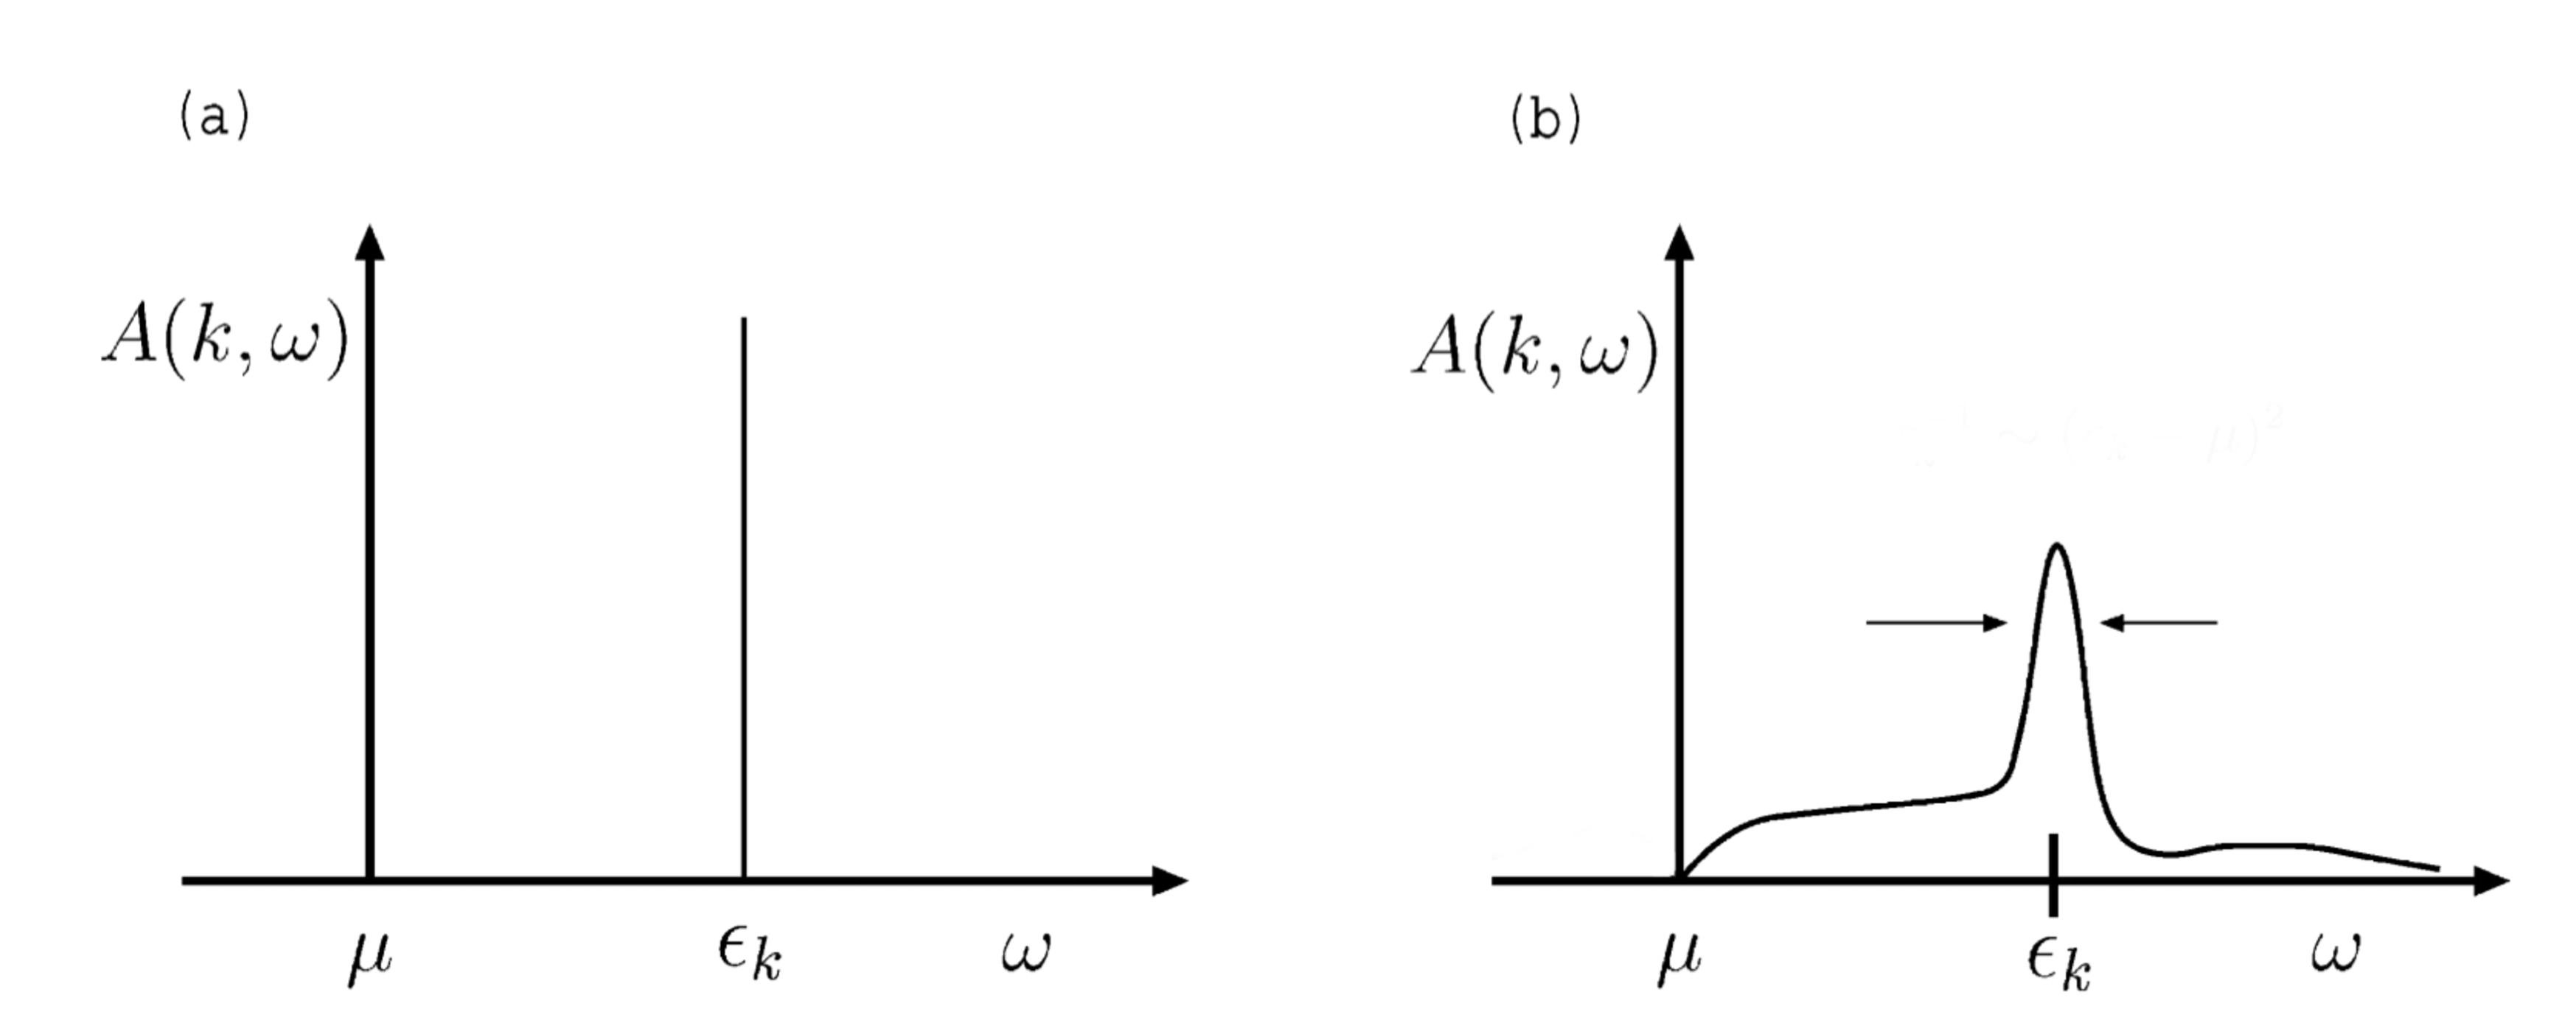
\includegraphics[width=0.8\linewidth]{fig1/flspectral.pdf}
    
\caption{The spectral function interacting and non-interacting system: (a) In a non-interacting system, electrons are eigenstates and so the probability is a $\delta$ function centred on the electron energy,
$\epsilon _k$. (b) In the Fermi liquid system, the probability is spread out with a peak at the new quasiparticle energy. Taken from Ref. \cite{Saarloos} with permission. \label{fig:flspectral}}
\end{figure} 



However, there are other materials which show new properties. These materials are known as non-Fermi liquid. Some examples of these systems are Heavy Fermions \cite{Stewart} and system of interacting fermions in one dimension which is called the Luttinger liquid \cite{Schulz}. Non-Fermi-liquid behaviour usually can be seen experimentally near a magnetically ordered phase in the phase diagram, which shows the non-Fermi-liquid state in the system may be related to a magnetic instability that appears at $T=0$ \cite{Stewart}. 



\section{Hubbard Model}
The Hubbard model was introduced in 1963 in two different papers, first by Gutzwiller \cite{Gutzwiller}, and then Hubbard \cite{Hubbard}. They tried to explain the effect of correlations for d-electrons in transition metals in a simple way\cite{Monto}. Different models have been proposed to study the many-body aspects of the electronic properties of condensed matter, but the Hubbard model is maybe the simplest model. This model tries to simplify the physics of matter by including only an effective local interaction. It means complexities of atomic physics and the corresponding multi-band description of condensed matter have been neglected\cite{Mario}. As mentioned one of the main motivations to study the Hubbard model is that, not only is it the simplest generalization beyond the band theory description of solids, but also it seems it can explain the main physical features of many systems. The Hubbard model has been used to describe\cite{Fabian}:
\begin{itemize}
    \item the electronic properties of solids with narrow bands,
    \item band magnetism in iron, cobalt, nickel,
    \item the Mott metal-insulator transition,
    \item electronic properties of $high-T_c$ cuprates in the normal state.
\end{itemize}
The Hamiltonian of the Hubbard model is:
\begin{equation}
\label{eqn:Hubbard}
H=-t\sum_{<i,i'>,\sigma}(c_{i,\sigma}^{\dagger}c_{i',\sigma}+c_{i',\sigma}^{\dagger}c_{i,\sigma})
+U\sum_{i=1}^Nn_{i\uparrow}n_{i\downarrow}.
\end{equation}

In this formula $i,i'$ label the sites of a D-dimensional lattice, $c_{i,\sigma}^{\dagger}(c_{i,\sigma})$ are creation(annihilation) operators which create (annihilate) an electron of spin $\sigma(\uparrow,\downarrow)$ on a site $i$, $n_{i\sigma}=c_{i,\sigma}^{\dagger}c_{i,\sigma}$ is an electron number operator which counts the number of electrons with spin $\sigma$ at site $i$. The first term in the Hubbard model Hamiltonian is chemical bonding and is known as "hopping" which represents a single particle interaction and hops an electron from one atom to the nearest neighbour atom with hopping matrix element $t$. The second term is related to two particle interaction, it explains the Coulomb repulsion between two electrons. The long-range contribution is neglected and only the interaction when both the electrons are on the same atom is retained, generating an energy of $U$ when the atom is doubly occupied \cite{Mario}. In Eq (\ref{eqn:Hubbard}) when $U>0$ it represents repulsive Coulomb interaction, and $U<0$ corresponds to an effective attractive interaction  between the electrons \cite{Monto}.

It is expected that Eq (\ref{eqn:Hubbard}) describes the main features of the materials, namely itinerant magnetism and metal-insulator (Mott) transition. When $U= 0$, $H$ reduces to a non-interacting system of moving electrons, and for $t= 0$ (atomic limit) the electrons are fully localized, and the system is insulator. In addition, for finite $t$ and $U =\infty$, the corresponding system is an antiferromagnetic insulator. \cite{Monto}.

Many efforts have been devoted to finding the solution of the Hubbard model. However, exact general solutions are not available, and existing solutions are mainly restricted to the one-dimensional case, in which there is no metal-insulator transition at any $T\neq0$. Even at $T = 0$ the exact solution doesn't show metal-insulator transition
for any $U > 0$. It is thought that the interplay between magnetic behaviour and the Mott transition near half-filling in the superconductors is crucial, since not only most of the new ceramic superconductors are good Mott insulators, but also they can show strong antiferromagnetic correlations, and the antiferromagnetic phase is close to the superconducting phase. It is shown that superconductivity can exist for U < 0, but for repulsive interaction it is not clear whether this is still true or not \cite{Monto}.
